\documentclass{beamer}
\mode<presentation> {
\usepackage{color}
\definecolor{bottomcolour}{rgb}{0.21,0.11,0.21}
\definecolor{middlecolour}{rgb}{0.21,0.11,0.21}
\setbeamercolor{structure}{fg=white}
\setbeamertemplate{frametitle}[default]%[center]
\setbeamercolor{normal text}{bg=black, fg=white}
\setbeamertemplate{background canvas}[vertical shading]
[bottom=bottomcolour, middle=middlecolour, top=black]
\setbeamertemplate{items}[circle]
\setbeamertemplate{navigation symbols}{} %no nav symbols
\setbeamercolor{block title}{use=structure,fg=white,bg=structure.fg!50!red!50!blue!100!green}
\setbeamercolor{block body}{parent=normal text,use=block title,bg=block title.bg!5!white!10!bg,fg=white}
\setbeamertemplate{navigation symbols}{}
}
\usepackage{graphicx} 
\usepackage{booktabs} 
\usepackage[utf8]{inputenc}  
\usepackage{geometry}     
%\usepackage[francais]{babel} 
\usepackage{eurosym}
\usepackage{verbatim}
\usepackage{ragged2e}
\justifying
%%%%%%%%%%%%%%%%%%%%%%%%%%%%%%%%%%%%%%%%%%%%%%%%%%%%%%%%%%%%%%%%
%% ccBeamer 0.1, 2007-07-02                                   %%
%% Written by Sebastian Pipping <webmaster@hartwork.org>      %%
%% ---------------------------------------------------------- %%
%% Licensed under Creative Commons Attribution-ShareAlike 3.0 %%
%% http://creativecommons.org/licenses/by-sa/3.0/             %%
%%%%%%%%%%%%%%%%%%%%%%%%%%%%%%%%%%%%%%%%%%%%%%%%%%%%%%%%%%%%%%%%


%% Images
\newcommand{\CcImageBy}[1]{%
	
\includegraphics[scale=#1]{creative_commons/cc_by_30.pdf}%
}
\newcommand{\CcImageCc}[1]{%
	
\includegraphics[scale=#1]{creative_commons/cc_cc_30.pdf}%
}
\newcommand{\CcImageDevNations}[1]{%
	
\includegraphics[scale=#1]{creative_commons/cc_dev_nations_30.pdf}%
}
\newcommand{\CcImageNc}[1]{%
	
\includegraphics[scale=#1]{creative_commons/cc_nc_30.pdf}%
}
\newcommand{\CcImageNd}[1]{%
	
\includegraphics[scale=#1]{creative_commons/cc_nd_30.pdf}%
}
\newcommand{\CcImagePd}[1]{%
	
\includegraphics[scale=#1]{creative_commons/cc_pd_30.pdf}%
}
\newcommand{\CcImageSa}[1]{%
	
\includegraphics[scale=#1]{creative_commons/cc_sa_30.pdf}%
}
\newcommand{\CcImageSampling}[1]{%
	
\includegraphics[scale=#1]{creative_commons/cc_sampling_30.pdf}%
}
\newcommand{\CcImageSamplingPlus}[1]{%
	
\includegraphics[scale=#1]{creative_commons/cc_sampling_plus_30.pdf}%
}


%% Groups
\newcommand{\CcGroupBy}[1]{% zoom
	\CcImageBy{#1}%
}
\newcommand{\CcGroupByNc}[2]{% zoom, gap
	\CcImageBy{#1}\hspace*{#2}\CcImageNc{#1}%
}
\newcommand{\CcGroupByNcNd}[2]{% zoom, gap
	\CcImageBy{#1}\hspace*{#2}\CcImageNc{#1}\hspace*{#2}\CcImageNd{#1}%
}
\newcommand{\CcGroupByNcSa}[2]{% zoom, gap
	\CcImageBy{#1}\hspace*{#2}\CcImageNc{#1}\hspace*{#2}\CcImageSa{#1}%
}
\newcommand{\CcGroupByNd}[2]{% zoom, gap
	\CcImageBy{#1}\hspace*{#2}\CcImageNd{#1}%
}
\newcommand{\CcGroupBySa}[2]{% zoom, gap
	\CcImageBy{#1}\hspace*{#2}\CcImageSa{#1}%
}
\newcommand{\CcGroupDevNations}[1]{% zoom
	\CcImageDevNations{#1}%
}
\newcommand{\CcGroupNcSampling}[2]{% zoom, gap
	\CcImageNc{#1}\hspace*{#2}\CcImageSampling{#1}%
}
\newcommand{\CcGroupPd}[1]{% zoom
	\CcImagePd{#1}%
}
\newcommand{\CcGroupSampling}[1]{% zoom
	\CcImageSampling{#1}%
}
\newcommand{\CcGroupSamplingPlus}[1]{% zoom
	\CcImageSamplingPlus{#1}%
}


%% Text
\newcommand{\CcLongnameBy}{Attribution}
\newcommand{\CcLongnameByNc}{Attribution-NonCommercial}
\newcommand{\CcLongnameByNcNd}{Attribution-NoDerivs}
\newcommand{\CcLongnameByNcSa}{Attribution-NonCommercial-ShareAlike}
\newcommand{\CcLongnameByNd}{Attribution-NoDerivs}
\newcommand{\CcLongnameBySa}{Attribution-ShareAlike}

\newcommand{\CcNote}[1]{% longname
	This work is licensed under the \textit{Creative Commons #1 3.0 License}.%
}

\title[Le logiciel libre]{Le logiciel libre} 
\author{Genma}
\begin{document}
%% Titlepage
\begin{frame}
	\titlepage
	\vfill
	\begin{center}
		\CcGroupByNcSa{0.83}{0.95ex}\\[2.5ex]
		{\tiny\CcNote{\CcLongnameByNcSa}}
		\vspace*{-2.5ex}
	\end{center}
\end{frame}
%-----------------------------------------------
\begin{frame}
\frametitle{Un logiciel, c'est quoi?}
\begin{block}{Définissions ce qu'est un logiciel}
\justifying{
Un logiciel, c'est un programme.
\\~\\ Pour qu'un ordinateur fonctionne, il a besoin d'un programme principal, que l'on appelle le système d'exploitation (Windows, Linux, MacOS X...) et de logiciels/programmes. 
\\~\\Il y des logiciels de bureautique (Word, Excel ou la suite LibreOffice), de traitement d'images, pour écouter de la musique ou voir des vidéos, aller sur Internet...
}
\end{block}
\end{frame}

%-----------------------------------------------
\begin{frame}
\frametitle{Le logiciel libre au quotidien}

\begin{block}{Le logiciel libre, est-ce réservé à des informaticiens?}
\begin{itemize}
\justifying{
\item Non, vous utilisez du logiciel libre tous les jours sans même le savoir. Par exemple, dans les box ADSL (Freebox etc), Android sont basés sur Linux.
\item Internet repose majoritairement sur des machines (les serveurs) qui font tournés les logiciels Apache/MYSQL/PHP qui sont des logiciels libres.
}
\end{itemize}
\end{block}
\end{frame}

\begin{frame}
\frametitle{Quelques logos de logiciels libres connus}

\includegraphics[scale=0.5] {./images/Le_logiciel_libre.png} 
\end{frame}

%-----------------------------------------------
\begin{frame}
\frametitle{Les principaux fondateurs}
\begin{columns}[c] 
\column{.55\textwidth} 
\begin{center}
Richard M.Stallman : les libertés du logiciel libre, le projet GNU
\\~\\

\includegraphics[scale=1] {./images/rms.jpg} 
\end{center}
\column{.5\textwidth} 
\begin{center}
Linus Torwalds : le noyau Linux \\~\\
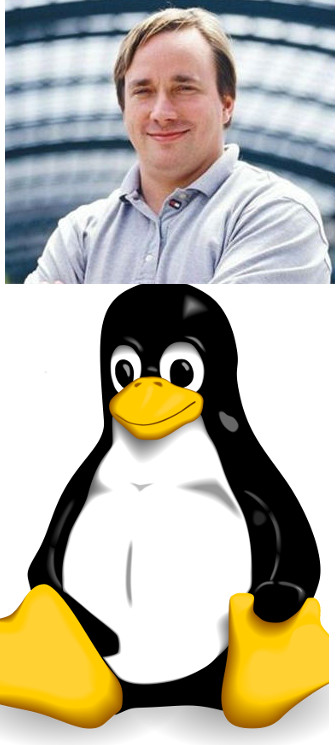
\includegraphics[scale=1] {./images/linux.jpg} 
\end{center}
\end{columns}
\end{frame}

%-----------------------------------------------
\begin{frame}
\begin{center}
\Huge{Et des millions d'autres personnes, chaque jour, depuis des dizaines d'années...}
\end{center}
\end{frame}

%-----------------------------------------------
\begin{frame}
\begin{center}
\Huge{Les 4 libertés}
\\~\\

\includegraphics[scale=1] {./images/gnu.jpg} 
\end{center}
\end{frame}

%-----------------------------------------------
\begin{frame}
\frametitle{4 libertés}
\begin{block}{Les 4 libertés du logiciel libre}
\begin{itemize}
\justifying{
\item la liberté d'utiliser le logiciel ;
\item la liberté de copier le logiciel ;
\item la liberté d'étudier le logiciel ;
\item la liberté de modifier le logiciel et de redistribuer les versions modifiées.
}
\end{itemize}
\end{block}
\end{frame}

%-----------------------------------------------
\begin{frame}
\begin{center}
\Huge{Pour mieux comprendre,\\ une analogie  avec \\les recettes de cuisine...}
\end{center}
\end{frame}

%-----------------------------------------------
\begin{frame}
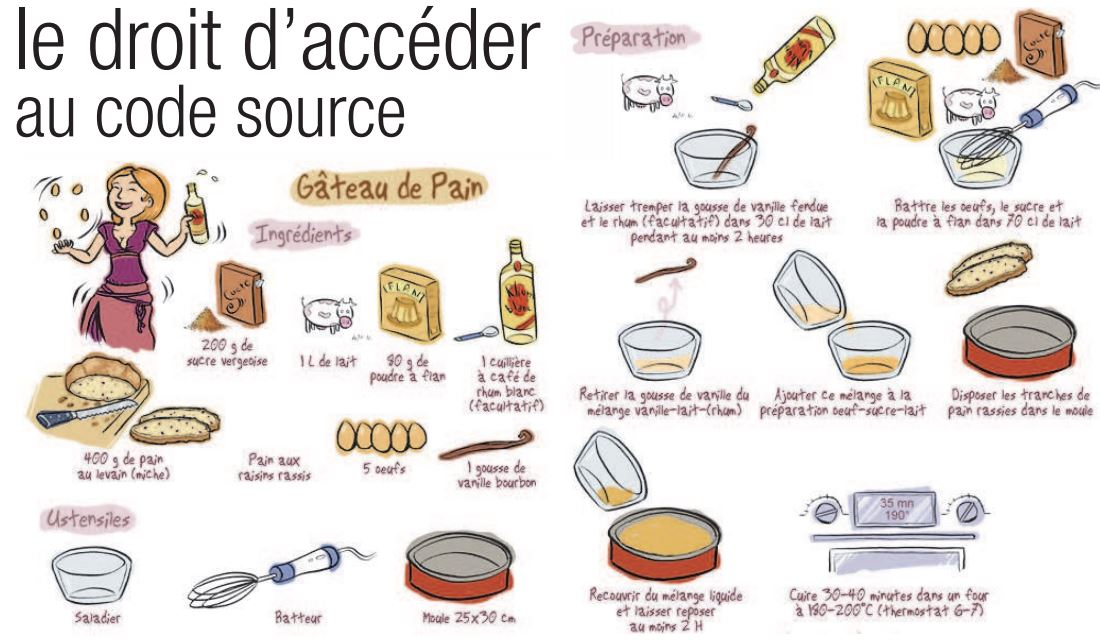
\includegraphics[scale=0.6] {./images/Cuisine01.jpg} 
\end{frame}
\begin{frame}
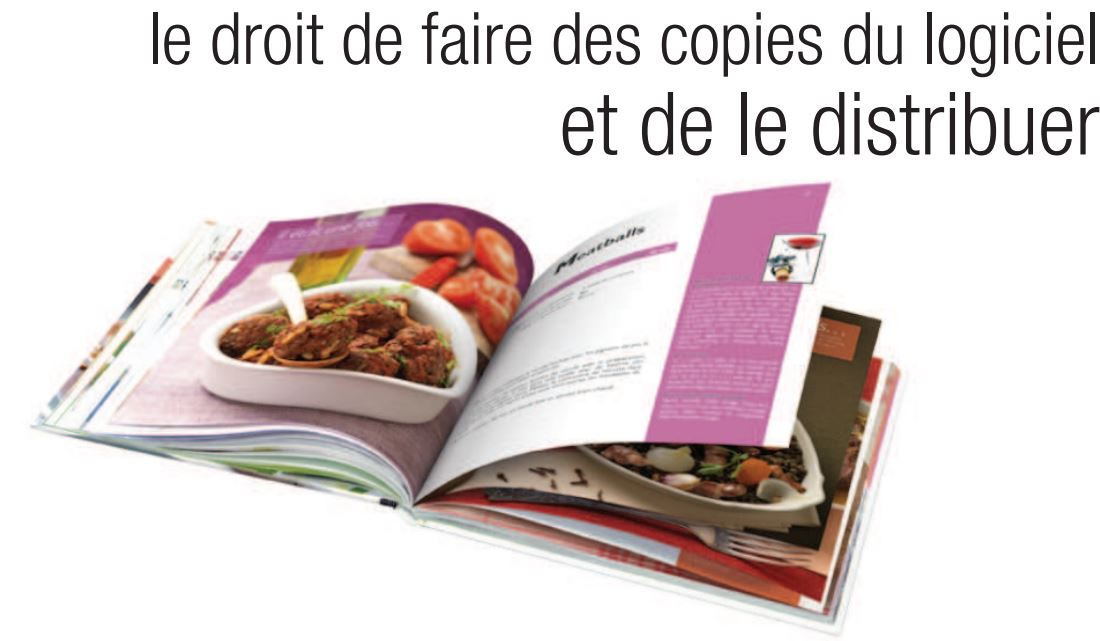
\includegraphics[scale=0.5] {./images/Cuisine02.jpg} 
\end{frame}
\begin{frame}
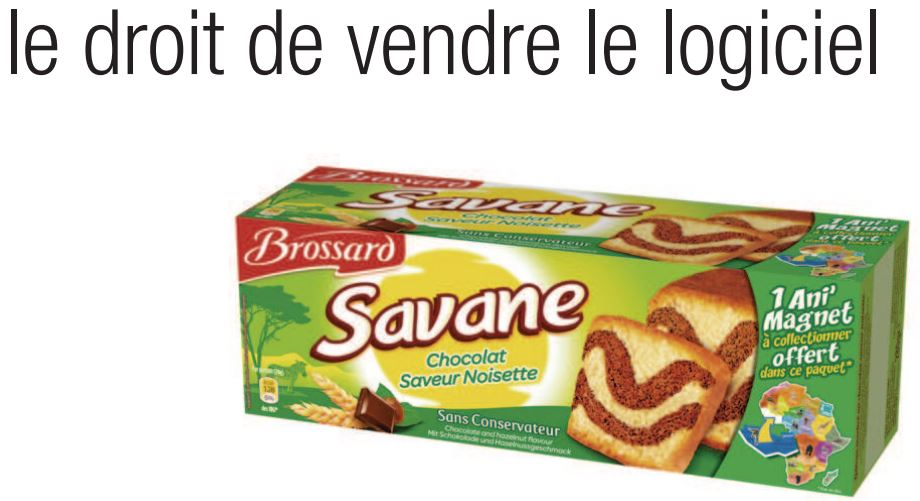
\includegraphics[scale=0.6] {./images/Cuisine03.jpg} 
\end{frame}
\begin{frame}
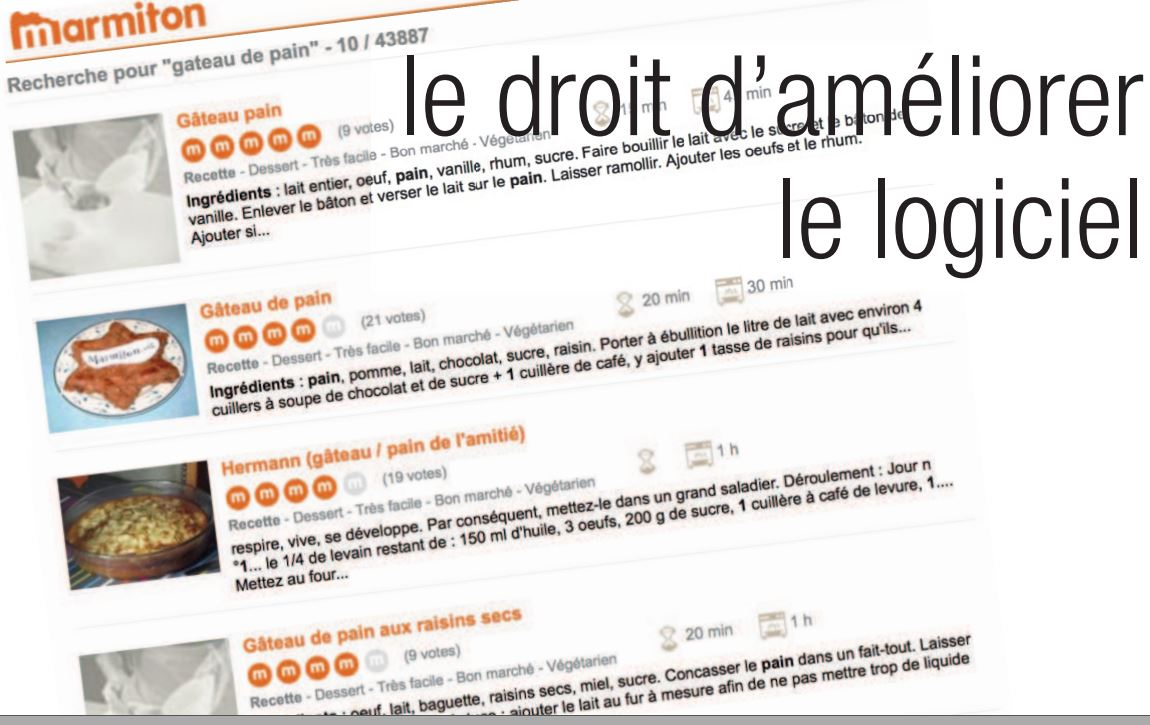
\includegraphics[scale=0.48] {./images/Cuisine04.jpg} 
\end{frame}

%-----------------------------------------------
\begin{frame}
\frametitle{C'est gratuit ou pas?}
\begin{block}{Free Software}
\begin{itemize}
\justifying{
\item  Free en anglais : deux sens. Libre ou gratuit.
\item \emph{Free as speach, not Free as beer}.
}
\end{itemize}
\justifying{
Le logiciel libre est très souvent disponible gratuitement.
\\Mais ce n'est pas une  \emph{obligation}.
}
\end{block}
\end{frame}

%-----------------------------------------------
\begin{frame}
\frametitle{Un peu de vocabulaire à retenir}

\begin{block}{Logiciel propriétaire/privateur}
\justifying{
Un logiciel aux sources fermées, on ne peut savoir ce qu'il fait exactement. Il faut faire confiance.
}
\end{block}
\begin{block}{Logiciel libre}
\justifying{
Un aspect philosophique, idéaliste...
}
\end{block}
\begin{block}{Open source}
\justifying{
Un aspect technique, un terme  \emph{commercial}...
}
\end{block}
\end{frame}

%-----------------------------------------------
\begin{frame}
\frametitle{La notion de licence au delà du logiciel}
\justifying{
Ces libertés se sont étendues au delà du logiciel.
}
\begin{block}{Licence Art libre}
\justifying{
On trouve des licences Art libre...
\\~\\
\begin{center}
 
\includegraphics[scale=1] {./images/Logo_Licence_Art_Libre.png} 
\end{center}
}
\end{block}

\begin{block}{Les Licences Creative Commons}
\begin{columns}[c] 
\column{.55\textwidth} 
\begin{center}
 
\includegraphics[scale=1] {./images/CC-by-sa.png}
\end{center}
\column{.5\textwidth} 
\begin{center}
 
\includegraphics[scale=1] {./images/CC-by-nc-sa.jpg} 
\end{center}
\end{columns}
 \end{block}
\end{frame}

%-----------------------------------------------
\begin{frame}
\begin{center}
\Huge{Les logiciels libres \\les plus populaires}
\end{center}
\end{frame}

%-----------------------------------------------
\begin{frame}
\frametitle{
\includegraphics[scale=0.2] {./images/libreoffice.png}~ Bureautique : LibreOffice}
\justifying{Dérivé d'OpenOffice, alternative à la suite Office (Word, Excel...)}
\begin{center}
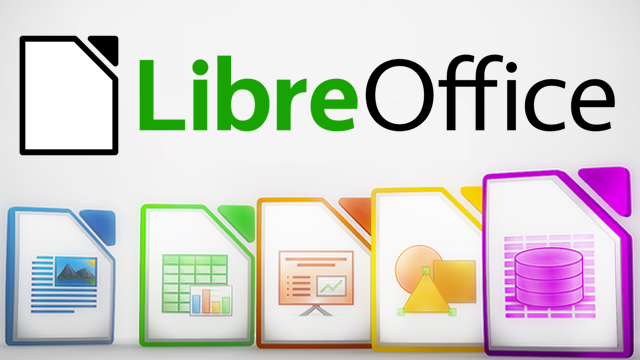
\includegraphics[scale=0.4] {./images/libreoffice_complet.png} 
\end{center}
\end{frame}

\begin{frame}
\frametitle{
\includegraphics[scale=0.2] {./images/gimp.png} ~ Retouche d'images: Gimp}
\justifying{
Alternative à Photoshop.
}
\begin{center}
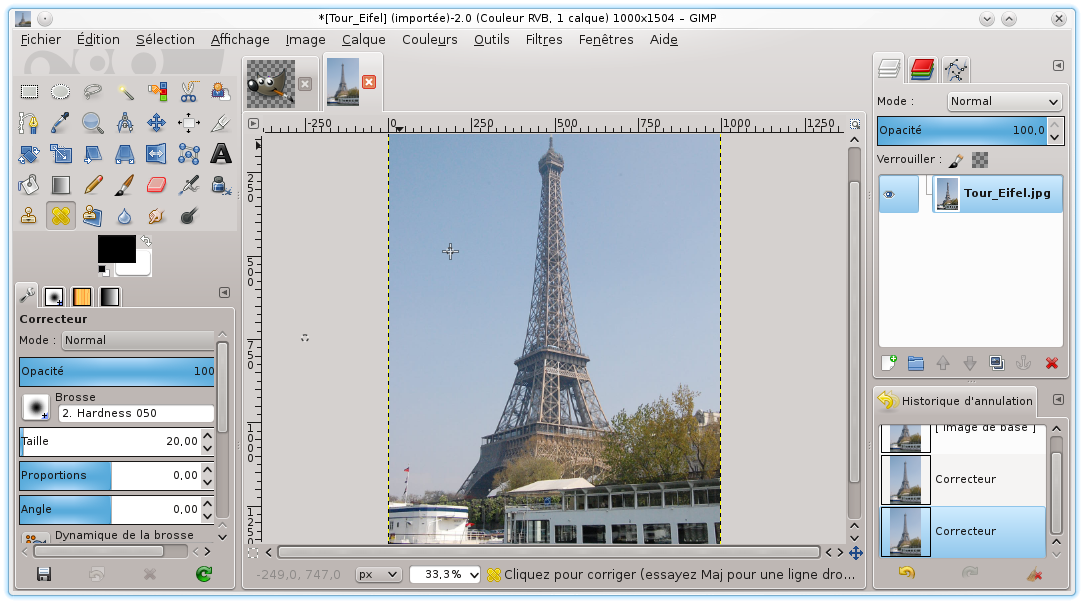
\includegraphics[scale=0.4] {./images/The_Gimp_in_action.png} 
\end{center}
\end{frame}

\begin{frame}
\frametitle{
\includegraphics[scale=0.1] {./images/firefox.png} ~  Navigateur : Firefox}
\begin{center}
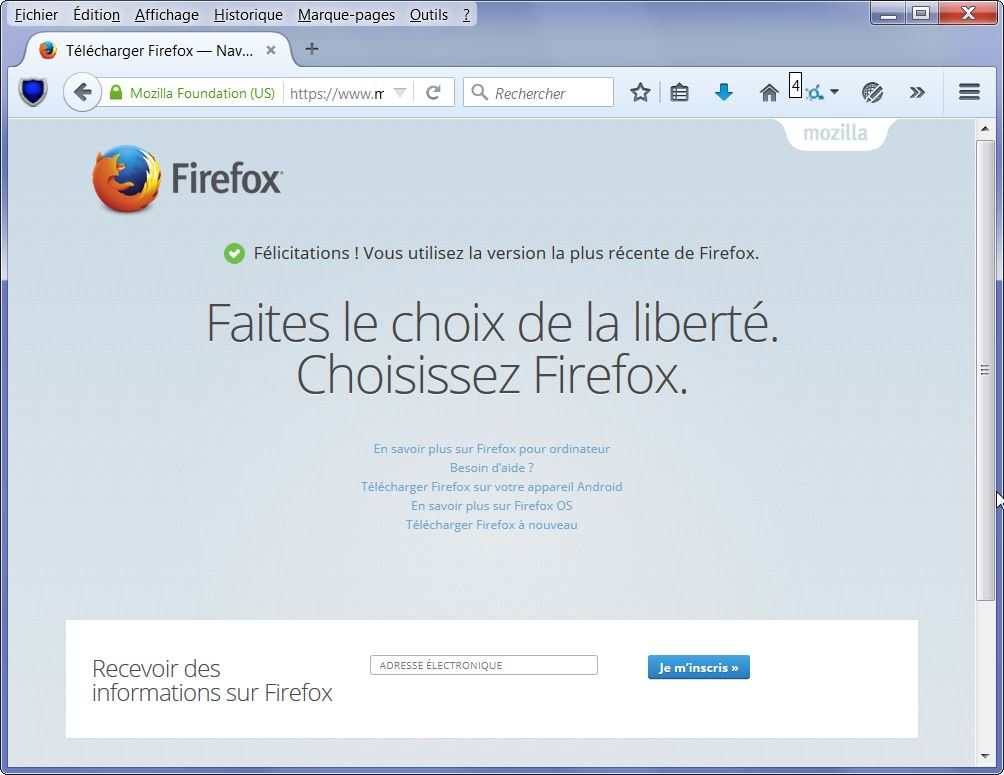
\includegraphics[scale=0.5] {./images/firefox_capture.jpg} 
\end{center}
\end{frame}

\begin{frame}
\frametitle{
\includegraphics[scale=0.05] {./images/vlc.png}  ~ Lecteur de vidéos : VLC}
\begin{center}
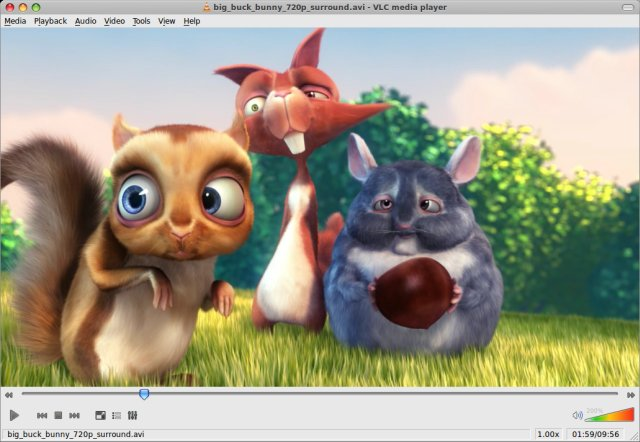
\includegraphics[scale=4] {./images/media-player-vlc-bunny.jpg} 
\end{center}
\end{frame}

\begin{frame}
\frametitle{
\includegraphics[scale=0.1] {./images/ubuntu.png} ~ Système complet : Ubuntu}
\begin{center}
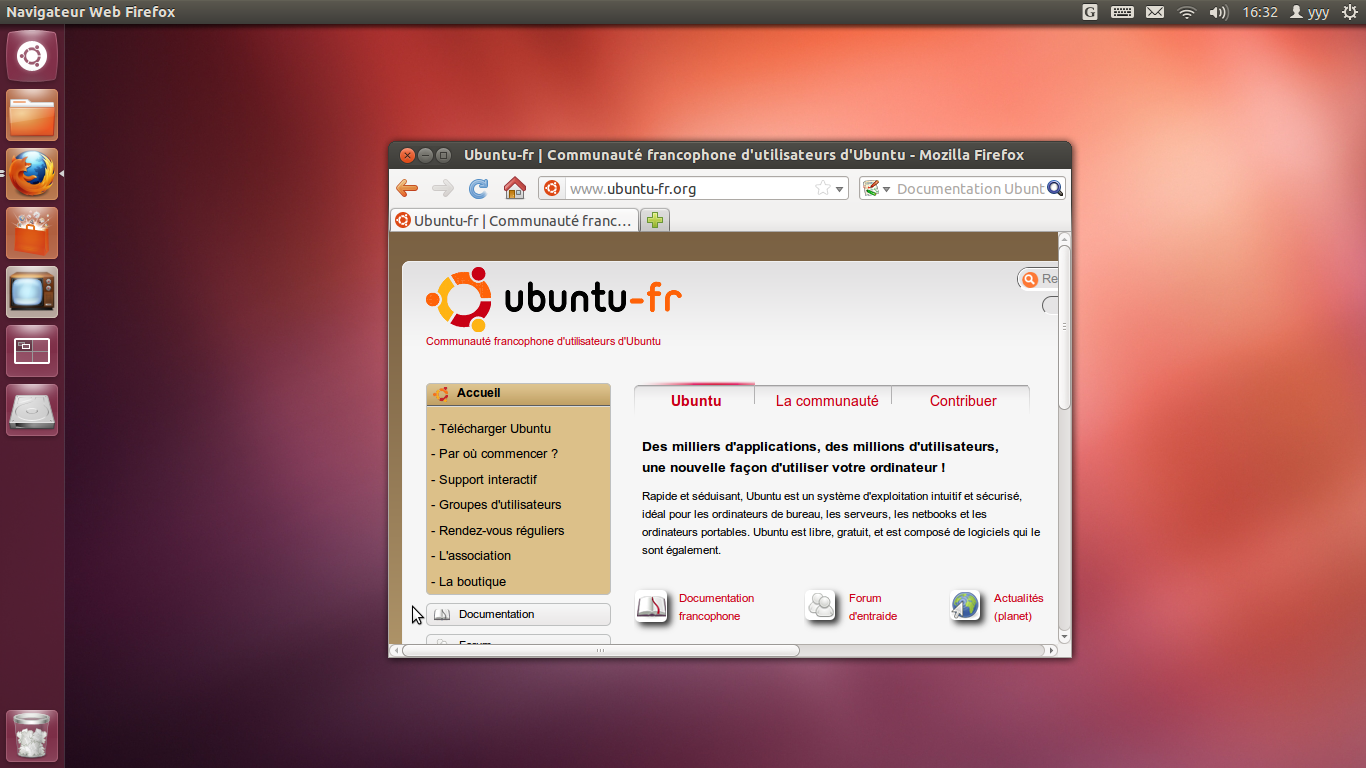
\includegraphics[scale=0.3] {./images/ubuntu_bureau.jpg} 
\end{center}
\end{frame}

%-----------------------------------------------
\begin{frame}
\begin{center}
\Huge{Et des milliers d'autres...
\\Voir \url{www.framasoft.net}}
\begin{center}
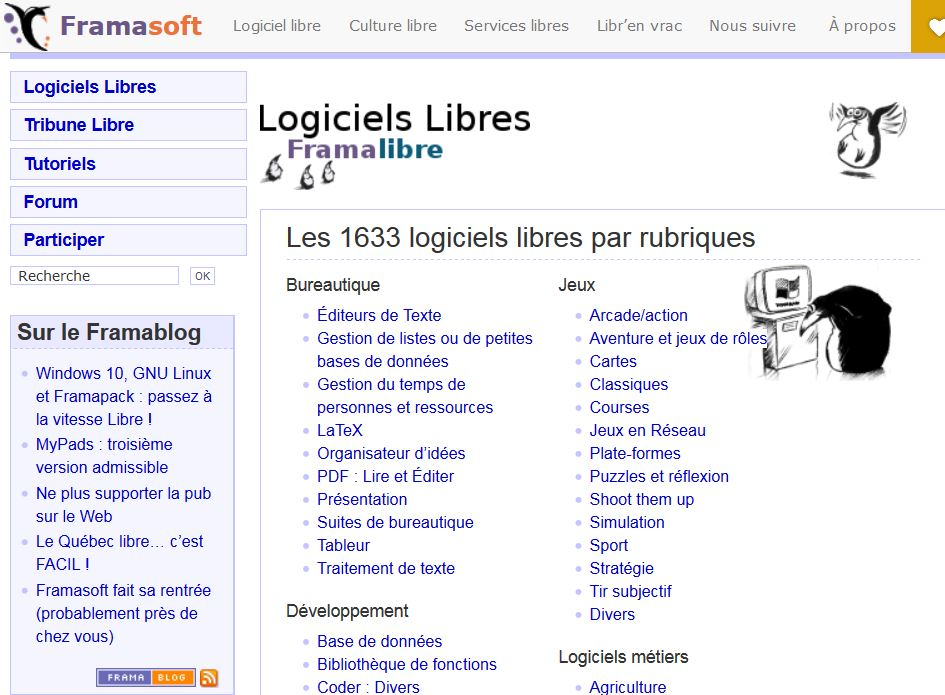
\includegraphics[scale=0.4] {./images/framasoft.jpg}
\end{center} 
\end{center}
\end{frame}

%-----------------------------------------------
\begin{frame}
\begin{center}
\Huge{Avantages et inconvénients}
\end{center}
\end{frame}

%-----------------------------------------------
\begin{frame}
\frametitle{Avantages}

\begin{block}{Les avantages du logiciel libre}
\begin{itemize}
\justifying{
\item adaptabilité : il est possible de réutiliser le code d'un logiciel libre pour créer un nouveau projet lorsque l'on a un besoin précis, plutôt que de repartir de 0,
\item la visibilité sur le cœur du logiciel, afin de s'assurer de sa fiabilité, sa qualité et sa sécurité,
\item la force d'une communauté ouverte par rapport à une équipe fermée, notamment concernant la rapidité de correction des éventuelles failles, et d'amélioration du logiciel,
\item la relative indépendance par rapport à des facteurs extérieurs, bien plus que pour des solutions propriétaires,
\item la qualité d'ensemble de ce genre de logiciels, dont le code peut être lu, relu et corrigé par de nombreux développeurs,
}
\end{itemize}
\end{block}
\end{frame}

%-----------------------------------------------
\begin{frame}
\frametitle{Inconvénients}

\begin{block}{Les inconvénients du logiciel libre}
\begin{itemize}
\justifying{
\item La multitude de choix (notion de fork) : on est perdu
\item L'accessibilité : logiciels qu'il faut réapprendre
\item Des gens passionnés : ils ne sont pas toujours pédagogues, il peut y avoir un \emph{élitisme technique}
\item La barrière de la langue (l'anglais est majoritaire)
\item L'accès à la documentation (ancienne et non à jour, incomplète, trop technique...)
}
\end{itemize}
\end{block}
\end{frame}

%-----------------------------------------------
\begin{frame}
\begin{center}
\Huge{Passer au logiciel libre?}\\~\\
\LARGE{Se faire installer "Linux ou Ubuntu..."}
\end{center}
\end{frame}

%-----------------------------------------------
\begin{frame}
\frametitle{Les associations}

\begin{block}{APRIL}
\justifying{
Pionnière du logiciel libre en France, l'April, constituée de 4248 adhérents est depuis 1996 un acteur majeur de la démocratisation et de la diffusion du logiciel libre et des standards ouverts auprès du grand public, des professionnels et des institutions dans l'espace francophone.
\url{http://www.april.org/}
}
\end{block}

\begin{center}

\includegraphics[scale=0.3] {./images/april.png}
\end{center} 
\end{frame}

\begin{frame}
\frametitle{Framasoft}
\begin{center}
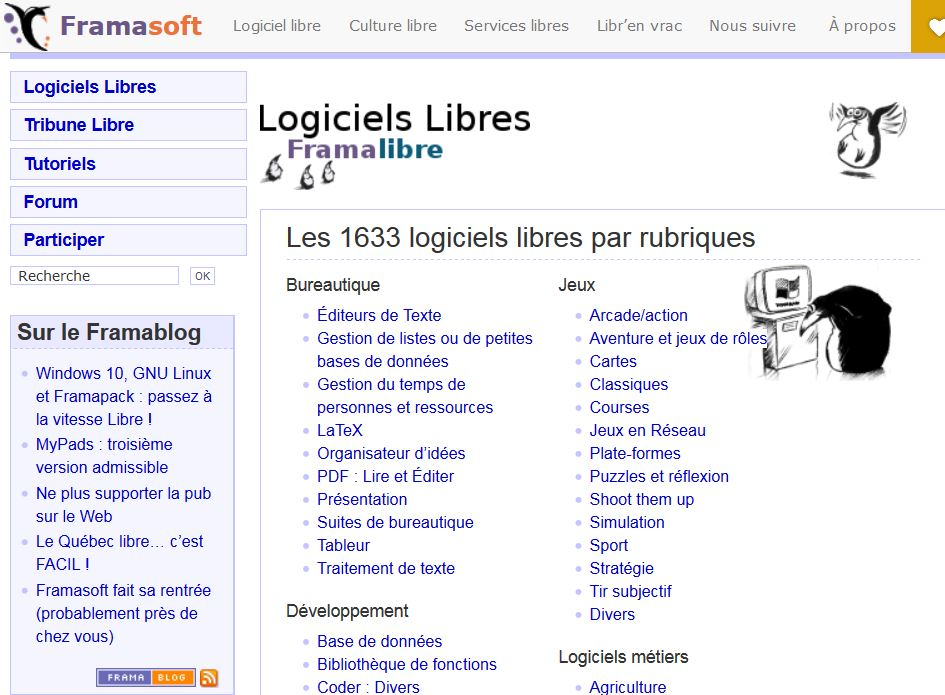
\includegraphics[scale=0.6] {./images/framasoft.jpg}
\end{center} 
\end{frame}
%-----------------------------------------------
\begin{frame}
\frametitle{Sur Paris - Parinux}

\begin{block}{Premier Samedi du Libre (PSL)}
\justifying{Chaque premier samedi de chaque mois, les bénévoles des associations du Libre vous accueillent au Carrefour Numérique de la Cité des sciences et de l'industrie (CSI) pour une install party.\\ \url{http://www.http://premier-samedi.org/}
}
\end{block}
\begin{center}

\includegraphics[scale=0.5] {./images/parinux.png}
\end{center} 
\end{frame}
%-----------------------------------------------
\begin{frame}
\frametitle{Sur Paris - Ubuntu Party}
\begin{block}{Ubuntu-fr}
Ubuntu Party : prochaine les 28 et 29 novembre à la CSI.\\
\url{http://www.ubuntu-paris.org/}
\end{block}
\begin{center}
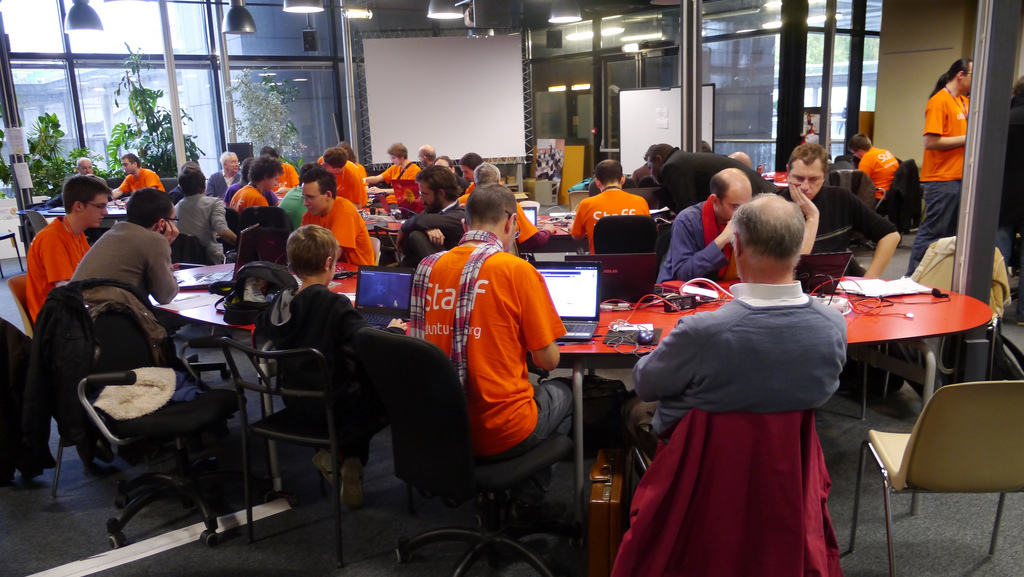
\includegraphics[scale=0.3] {./images/ubuntu-paris.jpg}
\end{center} 
\end{frame}
%-----------------------------------------------
\begin{frame}
\frametitle{Agenda}
Toutes les dates sont annoncées sur l'Agenda du libre 
\begin{center}
\url{http://www.agendadulibre.org/}
\\
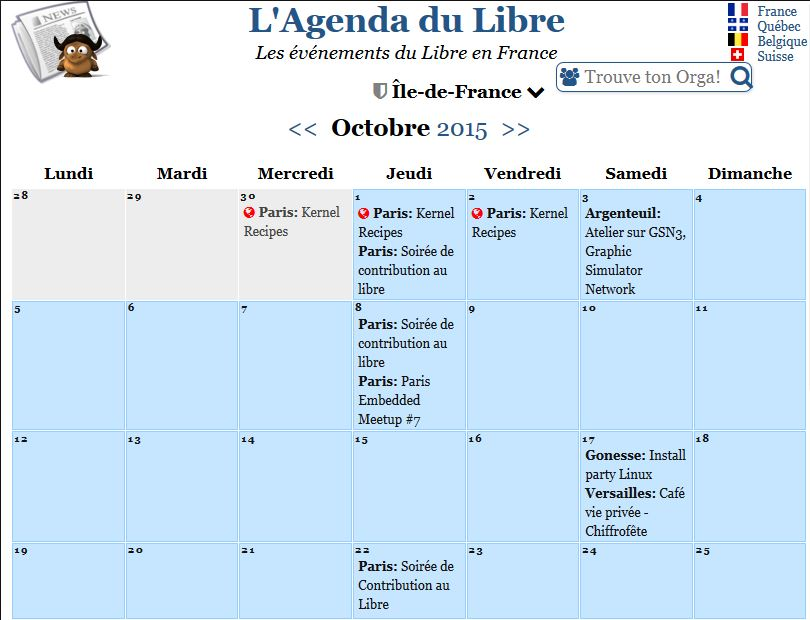
\includegraphics[scale=0.55] {./images/agenda-du-libre.jpg}
\end{center} 

\end{frame}
%----------------------------------------------------------------------------------------
\begin{frame}
\begin{center}
\Huge{Conclusion}
\end{center}
\end{frame}

%----------------------------------------------------------------------------------------
\begin{frame}
\begin{center}
\Huge{Merci de votre attention, \\place aux questions?}
\end{center}
\end{frame}

%----------------------------------------------------------------------------------------
\begin{frame}
\begin{center}
\Huge{Démonstration des logiciels libres via Ubuntu}
\end{center}
\end{frame}
\end{document}